\documentclass{article}

%-------------------------------------------------

\usepackage{fullpage}

\usepackage{graphicx}

\usepackage{amsmath}
\usepackage{amssymb}
\usepackage{amsfonts}

\usepackage{color}

\usepackage{verbatim}

\usepackage{tikz}
\usetikzlibrary{arrows,automata}

%-------------------------------------------------

\newcommand{\FIXME}[1]{\textcolor{red}{\textbf{#1}}}

%-------------------------------------------------

\newcommand{\stdin}{\texttt{stdin}~}
\newcommand{\stdout}{\texttt{stdout}~}
\newcommand{\stderr}{\texttt{stderr}~}

\newcommand{\multiprocessing}{\texttt{multiprocessing}~}
\newcommand{\multiprocessingConnection}{\texttt{multiprocessing.Connection}~}

\newcommand{\GraceDB}{\texttt{GraceDB}~}
\newcommand{\alert}{\texttt{lvalert}~}

\newcommand{\lvalertListen}{\texttt{lvalert\_listen}~}

\newcommand{\lvalertMP}{\texttt{lvalertMP}~}
\newcommand{\lvalertListenMP}{\texttt{lvalert\_listenMP}~}
\newcommand{\lvalertCommandMP}{\texttt{lvalert\_commandMP}~}

\newcommand{\interactiveQueue}{\texttt{interactiveQueue}~}
\newcommand{\parseAlert}{\texttt{parseAlert}~}

\newcommand{\SortedQueue}{\texttt{SortedQueue}~}
\newcommand{\QueueItem}{\texttt{QueueItem}~}
\newcommand{\Task}{\texttt{Task}~}

\newcommand{\lvalertMPini}{\texttt{lvalert\_listenMP.ini}~}
\newcommand{\childConfigini}{\texttt{childConfig.ini}~}

\newcommand{\approvalProcessor}{\texttt{approval\_processor}~}
\newcommand{\eventSupervisor}{\texttt{event\_supervisor}~}

%-------------------------------------------------
\begin{document}
%-------------------------------------------------

\title{
\lvalertMP User's Guide
}

\author{
Reed Essick \\
reed.essick@ligo.org
}

\maketitle

\newpage

%------------------------

\tableofcontents
\listoffigures

\newpage

%------------------------

\section{introduction}

\lvalertListen provides an extremely flexible infrastructure from which processes can listen and respond to events within \GraceDB. 
However, it currently only communicates with the forked process once (via \stdin) and therefore cannot send multiple \alert messages to any procesess.
For most follow-up, this is not an issue.
Many processes simply respond to any new event which passes a basic FAR threshold. 
However, a few key processes will benefit from receiving all alerts about a set of events.
Indeed, passing all \alert messages to a single process obviates the inter-process communication and associated race conditions that would be required of multiple independent processes, each forked with a separate, single \alert message.

This guide describes how \lvalertListenMP addresses and resolves this problem. 
In particular, we focus on a pedagogical description of the classes and methods used within the executables.
We also focus on the user's interface with the tools from the command line.

Briefly, \lvalertListenMP uses the same interface with the \alert servers but forks child processes via Pythons multiprocessing module.
In this way, \lvalertListenMP can communciate with the child processes repeatedly (through a shared \multiprocessingConnection object).
The module provides a standardized way to schedule and execute follow-up activities.
While the actual follow-up implemented here is basic, it is easily extended to achieve more complicated goals.
An example is the \eventSupervisor library.

This guide is organized as follows. In \S\ref{sec: classes, methods, configs and executables}, we enumerate and describe the basic objects, methods, configuration files and executables defined within this module. 
This includes examples for how these might be used.
In \S\ref{sec: workflow}, we demonstrate the workflow within \lvalertListenMP and describe how the various parts work together to manage follow-up tasks.
Finally, we discuss existing and suggested extensions in \S\ref{sec: suggested extensions}.

%------------------------

\section{classes, methods, configs and executables}
\label{sec: classes, methods, configs and executables}

This section defines the classes (\S\ref{sec: classes}), methods (\S\ref{sec: methods}), configuration files (\S\ref{sec: configs}), and executables (\S\ref{sec: executables}) that are necessary for \lvalertListenMP to function. 
Their interactions are described in \S\ref{sec: workflow}, so we focus on the particular responsibilities associated with each element here.

%-----------

\subsection{classes}
\label{sec: classes}

There are three (3) main classes defined within \lvalertMP:
\begin{itemize}
    \item{\SortedQueue (\S\ref{sec: SortedQueue})}
    \item{\QueueItem (\S\ref{sec: QueueItem})}
    \item{\Task (\S\ref{sec: Task})}
\end{itemize}
These objects are what allow \lvalertListenMP to define and schedule multiple follow-up activities based on \alert messages about multiple events within a single process.
In particular, individual activities are encapsulated as \Task objects.
Each \QueueItem is associated with one or more \Task objects.
\SortedQueue contains an ordered list of \QueueItem instances, and when each \QueueItem \textit{expires} the activities associated therewith are accomplished through a call to \QueueItem.execute(), which in turn delegates to \Task.execute() for each associated \Task instance as needed.
Futhermore, \QueueItem instances posses the concept of ``completion'' and will label themselves as ``completed'' when all their \Task instances have been run.

%---

\subsubsection{\SortedQueue}
\label{sec: SortedQueue}

The \SortedQueue class is a simple wrapper around a Python \texttt{list} that manages the order of the elements within the \texttt{list}.
We require all elements to be a subclass of \QueueItem and so ensure that each element has a notion of \textit{expiration}.
Furthermore, \SortedQueue supports a few basic \texttt{list} manipulations and queries.

\vspace{0.5cm}
\noindent
\textit{attributes}

\begin{itemize}
    \item{queue [\texttt{list}]
        \begin{itemize}
            \item{a Python \texttt{list} which stores the \QueueItem instances. \SortedQueue orders the elements of this \texttt{list} and provides some high level interface functionality to manipulate them.}
        \end{itemize}
         }
\end{itemize}

\noindent
\textit{methods}

\begin{itemize}
    \item{\_\_init\_\_()
        \begin{itemize}
            \item{basic instantiation. Sets the \textit{queue} attribute to an empty list.}
        \end{itemize}
         }
    \item{\_\_len\_\_()
        \begin{itemize}
            \item{returns the length of the \texttt{list} stored as the \textit{queue} attribute.}
        \end{itemize}
         }
    \item{\_\_getitem\_\_(ind [\texttt{int}])
        \begin{itemize}
            \item{returns the element of \textit{queue} corresponding to a specified index.}
        \end{itemize}
         }
    \item{insert(newItem [\QueueItem])
        \begin{itemize}
            \item{inserts the new \QueueItem into \textit{queue} in the correct order. This is done through a direct integration over \textit{queue} and could be sped up by representing \textit{queue} with a better data structure. Also checks that the new \texttt{list} item is a sublcass of \QueueItem.}
        \end{itemize}
         }
    \item{pop(ind=0 [\texttt{int}])
        \begin{itemize}
            \item{removes and returns the \QueueItem corresponding the the specified index. The default is to return the first item in \textit{queue}.}
        \end{itemize}
         }
    \item{clean()
        \begin{itemize}
            \item{removes all \QueueItem instances marked as \textit{completed} from \textit{queue}. This allows us to simply modify an attribute of a \QueueItem upon execution or during \parseAlert (\S\ref{sec: parseAlert}) and let the \SortedQueue clean up all completed items periodically.}
        \end{itemize}
         }
\end{itemize}


%---

\newpage

\FIXME{left off here!}

\newpage

\subsubsection{\QueueItem}
\label{sec: QueueItem}

The \QueueItem class encapsulates the idea of a single follow-up process.
Each processes may be required to do several things and must order or schedule those things internally.
\QueueItem instances accomplish this by storing two \texttt{list}s of \Task objects, with each \Task respresenting a single activity.
As the \Task instances are completed (via delegation through \Task.execute), they are shuffled from the \textit{tasks} list to the \textit{completedTasks} list.
\QueueItem's also contain the concepts of \textit{expiration} (when the next \Task should be executed) as well as \textit{completion} (whether there are more tasks to be completed).
We note that the internal storage of ordered \Task instances within the \QueueItem is extremely similar to the ordered storage within \SortedQueue instances.
If desired, multiple \Task instances can be scheuduled and managed with \SortedQueue alone by assigning a single \Task to each \QueueItem and filling the \SortedQueue with multiple \QueueItem instances.
However, we allow \QueueItem instances to manage multiple tasks because this can sometimes simplify the representation of single follow-up processes.

\vspace{0.5cm}
\noindent
\textit{attributes}

\begin{itemize}
    \item{name [\texttt{str}]
        \begin{itemize}
            \item{}
        \end{itemize}
         }
    \item{description [\texttt{str}]
        \begin{itemize}
            \item{}
        \end{itemize}
         }
    \item{t0 [\texttt{float}]
        \begin{itemize}
            \item{}
        \end{itemize}
         }
    \item{tasks [\texttt{list}]
        \begin{itemize}
            \item{}
        \end{itemize}
         }
    \item{completedTasks [\texttt{list}]
        \begin{itemize}
            \item{}
        \end{itemize}
         }
    \item{expiration [texttt{float}]
        \begin{itemize}
            \item{}
        \end{itemize}
         }
\end{itemize}

\noindent
\textit{methods}

\begin{itemize}
    \item{\_\_init\_\_(t0 [\texttt{float}], tasks [\texttt{list}])
        \begin{itemize}
            \item{}
        \end{itemize}
         }
    \item{sortTasks()
        \begin{itemize}
            \item{}
        \end{itemize}
         }
    \item{hasExpired()
        \begin{itemize}
            \item{}
        \end{itemize}
         }
    \item{execute(verbose=False [\texttt{bool}])
        \begin{itemize}
            \item{}
        \end{itemize}
         }
    \item{add(newTasks [\texttt{list}])
        \begin{itemize}
            \item{}
        \end{itemize}
         }
    \item{remove(taskName [\texttt{str}])
        \begin{itemize}
            \item{}
        \end{itemize}
         }
\end{itemize}

%---

\subsubsection{\Task}
\label{sec: Task}

Each \Task represents one follow-up activity.
Each follow-up process may perform multiple activities and therefore correspond to multiple \Task objects.
These are grouped together under a single \QueueItem instance for each follow-up process.

\Task instances peform the actual follow-up activities through delegation and to their \textit{functionHandle} attributes.
There is a standardized input argument format for \textit{functionHandle} calls which is followed by the \Task.execute call.
This can be changed and/or modified by creating an extension of the \Task and overwriting the execute method.

\Task objects also contain the concept of \textit{timing out} and \textit{expiration}.
When they are instantiated, they only know of their \textit{timeout}, or the number of seconds (after some reference time) which must ellapse before they should be executed.
When the \textit{setExpiration} method is called, the \textit{expiration} time is computed using the supplied reference time to compute a global time-stamp.
Note, if we can call \textit{setExpiration} repeatedly if needed.

\vspace{0.5cm}
\noindent
\textit{attributes}

\begin{itemize}
    \item{name [\texttt{str}]
        \begin{itemize}
            \item{}
        \end{itemize}
         }
    \item{description [\texttt{str}]
        \begin{itemize}
            \item{}
        \end{itemize}
         }
    \item{timeout [\texttt{float}]
        \begin{itemize}
            \item{}
        \end{itemize}
         }
    \item{expiration [\texttt{float}]
        \begin{itemize}
            \item{}
        \end{itemize}
         }
    \item{functionHandle [\texttt{method}]
        \begin{itemize}
            \item{}
        \end{itemize}
         }
    \item{*args [\texttt{list}]
        \begin{itemize}
            \item{}
        \end{itemize}
         }
    \item{**kwargs [\texttt{dict}]
        \begin{itemize}
            \item{}
        \end{itemize}
         }
\end{itemize}

\noindent
\textit{methods}

\begin{itemize}
    \item{\_\_init\_\_(timeout [\texttt{float}], functionHandle [\texttt{method}], *args, **kwargs)
        \begin{itemize}
            \item{}
        \end{itemize}
         }
    \item{setExpiration(t0 [\texttt{float}])
        \begin{itemize}
            \item{}
        \end{itemize}
         }
    \item{hasExpired()
        \begin{itemize}
            \item{}
        \end{itemize}
         }
    \item{execute(graceid [\texttt{str}], gdb [\texttt{GraceDb}], verbose=False [\texttt{bool}], annotate=False [\texttt{bool}])
        \begin{itemize}
            \item{}
        \end{itemize}
         }
\end{itemize}

%-----------

\subsection{methods}
\label{sec: methods}

\begin{itemize}
    \item{\interactiveQueue (\S\ref{sec: interactiveQueue})}
    \item{\parseAlert (\S\ref{sec: parseAlert})}
\end{itemize}

%---

\subsubsection{\interactiveQueue}
\label{sec: interactiveQueue}

\vspace{0.5cm}
\noindent
\textit{arguments}

\begin{itemize}
    \item{connection
        \begin{itemize}
            \item{}
        \end{itemize}
         }
    \item{config
        \begin{itemize}
            \item{}
        \end{itemize}
         }
    \item{verbose
        \begin{itemize}
            \item{}
        \end{itemize}
         }
    \item{sleep
        \begin{itemize}
            \item{}
        \end{itemize}
         }
    \item{maxComplete
        \begin{itemize}
            \item{}
        \end{itemize}
         }
    \item{maxFrac
        \begin{itemize}
            \item{}
        \end{itemize}
         }
\end{itemize}

\noindent
\textit{key internal variables}

\begin{itemize}
    \item{queue
        \begin{itemize}
            \item{}
        \end{itemize}
         }
    \item{queueByGraceID
        \begin{itemize}
            \item{}
        \end{itemize}
         }
    \item{complete
        \begin{itemize}
            \item{}
        \end{itemize}
         }
    \item{process\_type
        \begin{itemize}
            \item{}
        \end{itemize}
         }
\end{itemize}

%---

\subsubsection{\parseAlert}
\label{sec: parseAlert}

\vspace{0.5cm}
\noindent
\textit{arguments}

\begin{itemize}
    \item{queue
        \begin{itemize}
            \item{}
        \end{itemize}
         }
    \item{queueByGraceID
        \begin{itemize}
            \item{}
        \end{itemize}
         }
    \item{alert
        \begin{itemize}
            \item{}
        \end{itemize}
         }
    \item{t0
        \begin{itemize}
            \item{}
        \end{itemize}
         }
    \item{config
        \begin{itemize}
            \item{}
        \end{itemize}
         }
    \item{timeout
        \begin{itemize}
            \item{}
        \end{itemize}
         }
\end{itemize}

\noindent
\textit{key internal variables}

\FIXME{what do we put here? This depends strongly on the process\_type.}

%-----------

\subsection{configs}
\label{sec: configs}

\begin{itemize}
    \item{\lvalertMPini (\S\ref{sec: lvalertMPini})}
    \item{\childConfigini (\S\ref{sec: childConfigini})}
\end{itemize}

%---

\subsubsection{\lvalertMPini}
\label{sec: lvalertMPini}

%---

\subsubsection{\childConfigini}
\label{sec: childConfigini}

%-----------

\subsection{executables}
\label{sec: executables}

\begin{itemize}
    \item{\lvalertListenMP (\S\ref{sec: lvalertListenMP})}
    \item{\lvalertCommandMP (\S\ref{sec: lvalertCommandMP})}
\end{itemize}

%---

\subsubsection{\lvalertListenMP}
\label{sec: lvalertListenMP}

\vspace{0.5cm}
\noindent
\textit{options}

\begin{itemize}
    \item{username
        \begin{itemize}
            \item{}
        \end{itemize}
         }
    \item{password (\FIXME{FIXME! support \texttt{.netrc} instead of \texttt{--password} option.)}
        \begin{itemize}
            \item{}
        \end{itemize}
         }
    \item{server
        \begin{itemize}
            \item{}
        \end{itemize}
         }
    \item{resource
        \begin{itemize}
            \item{}
        \end{itemize}
         }
    \item{config-file
        \begin{itemize}
            \item{}
        \end{itemize}
         }
    \item{show
        \begin{itemize}
            \item{}
        \end{itemize}
         }
    \item{node
        \begin{itemize}
            \item{}
        \end{itemize}
         }
    \item{verbose
        \begin{itemize}
            \item{}
        \end{itemize}
         }
    \item{debug
        \begin{itemize}
            \item{}
        \end{itemize}
         }
    \item{version
        \begin{itemize}
            \item{}
        \end{itemize}
         }
\end{itemize}

%---

\subsubsection{\lvalertCommandMP}
\label{sec: lvalertCommandMP}

\FIXME{WRITE this executable and document it here!}

\vspace{0.5cm}
\noindent
\textit{options}

%------------------------

\section{workflow}
\label{sec: workflow}

\begin{itemize}
    \item{how \alert messages are passed from the server to the separate (child) processes}
    \item{workflow within \interactiveQueue and how this manages the \SortedQueue instances}
    \item{workflow within \parseAlert and what this is responsible for}
\end{itemize}

\begin{figure}
    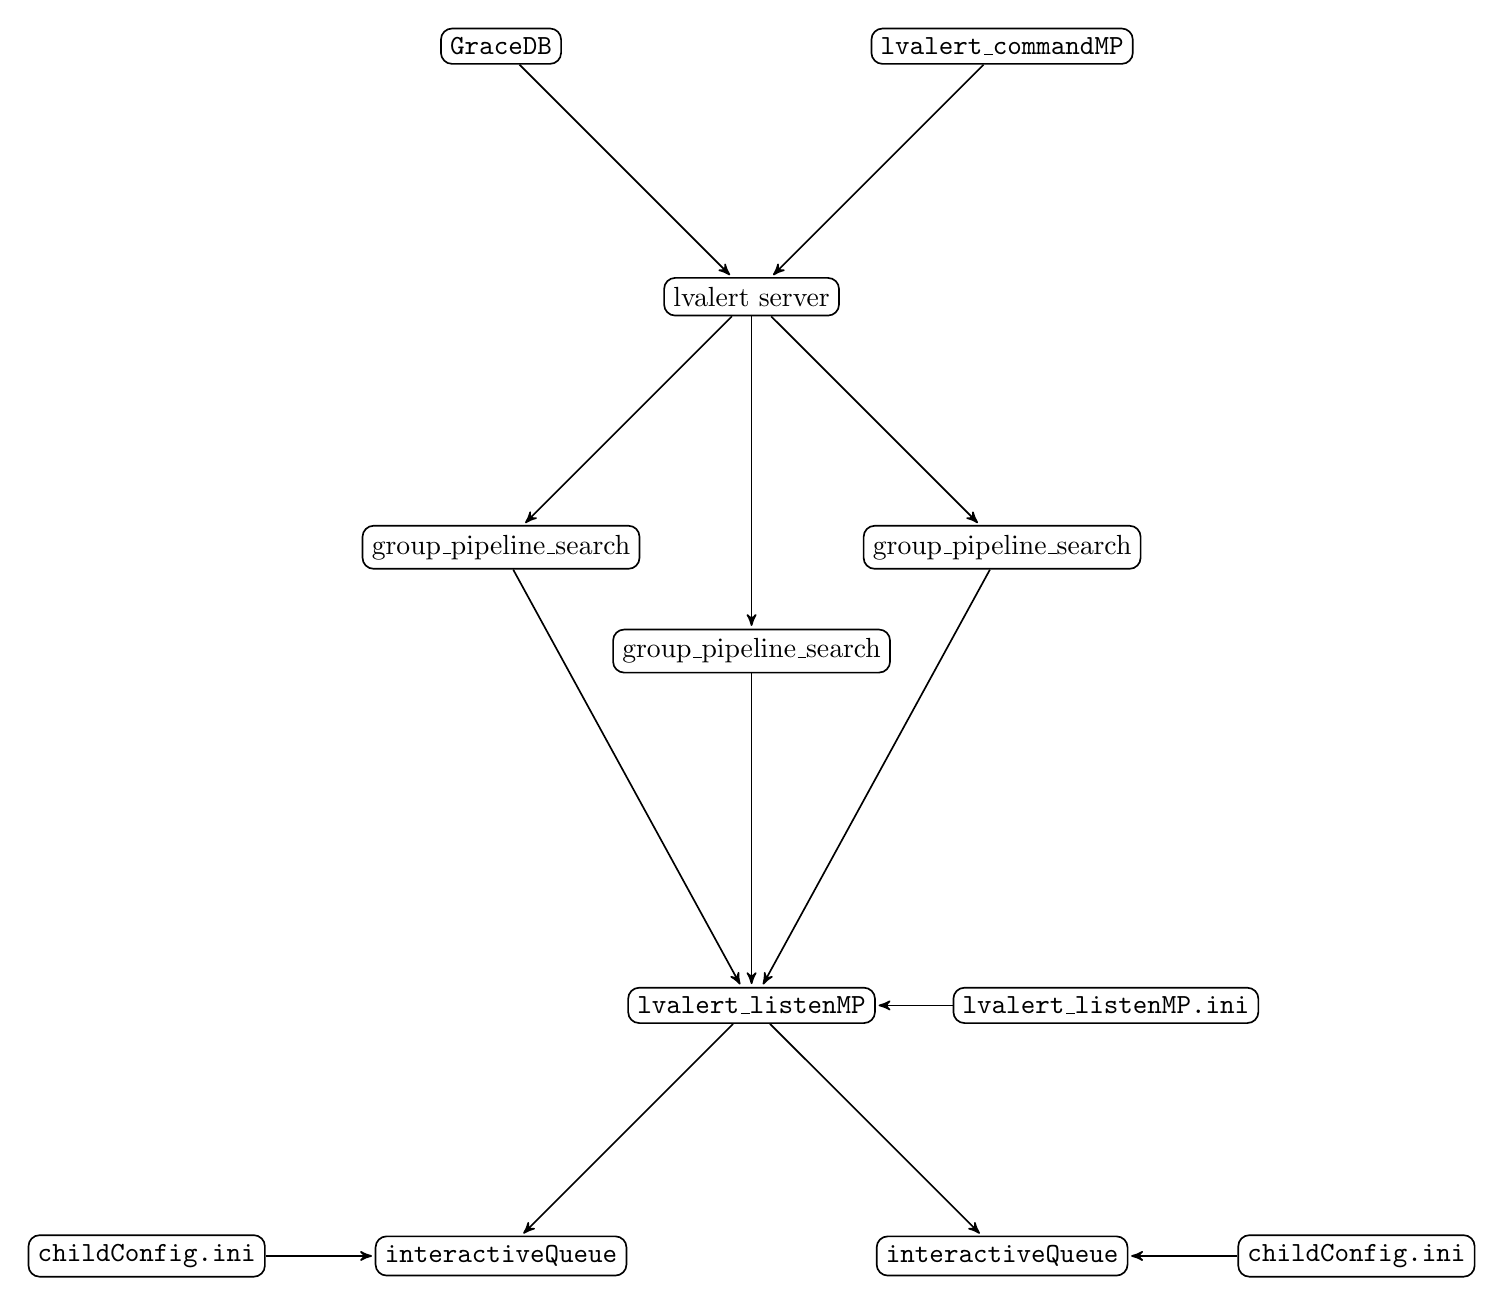
\begin{tikzpicture}[->,>=stealth', shorten >= 1pt, auto, node distance=4.50cm, semithick]
        \tikzset{
           server/.style={
                        rectangle,
                        rounded corners,
                        draw=black,
                        fill=none,
                        text=black
                       },
           lvalertNode/.style={
                        rectangle,
                        rounded corners,
                        draw=black,
                        fill=none,
                        text=black
                       },
           mpPipe/.style={
                        rectangle,
                        rounded corners,
                        draw=black,
                        fill=none,
                        text=black
                       },
           lvalertMP/.style={
                        rectangle,
                        rounded corners,
                        draw=black,
                        fill=none,
                        text=black
                       },
           config/.style={
                        rectangle,
                        rounded corners,
                        draw=black,
                        fill=none,
                        text=black
                       },
           childProc/.style={
                        rectangle,
                        rounded corners,
                        draw=black,
                        fill=none,
                        text=black
                       },
                 };
    %--------------------
        \node[server]      (lvalertServer)                                {lvalert server};

        \node[server]      (GraceDB)       [above left of=lvalertServer]  {\GraceDB};
        \node[lvalertMP]   (lvalertCmd)    [above right of=lvalertServer] {\lvalertCommandMP};

        \node[lvalertNode] (nodeA)         [below left of=lvalertServer]  {group\_pipeline\_search};
        \node[lvalertNode] (nodeB)         [below of=lvalertServer]       {group\_pipeline\_search};
        \node[lvalertNode] (nodeC)         [below right of=lvalertServer] {group\_pipeline\_search};

        \node[lvalertMP]   (lvalertMP)     [below of=nodeB]               {\lvalertListenMP};
        \node[config]      (lvalertConfig) [right of=lvalertMP]           {\lvalertMPini};

        \node[childProc]   (childProc1)    [below left of=lvalertMP]      {\interactiveQueue};
        \node[config]      (childConfig1)  [left of=childProc1]           {\childConfigini};
        \node[childProc]   (childProc2)    [below right of=lvalertMP]     {\interactiveQueue};
        \node[config]      (childConfig2)  [right of=childProc2]          {\childConfigini};
    %--------------------
        \path (GraceDB)       edge (lvalertServer)
              (lvalertCmd)    edge (lvalertServer)

              (lvalertServer) edge (nodeA)
              (lvalertServer) edge (nodeB)
              (lvalertServer) edge (nodeC)

              (nodeA)         edge (lvalertMP)
              (nodeB)         edge (lvalertMP)
              (nodeC)         edge (lvalertMP)

              (lvalertConfig) edge (lvalertMP)

              (lvalertMP)     edge (childProc1)
              (lvalertMP)     edge (childProc2)

              (childConfig1)  edge (childProc1)
              (childConfig2)  edge (childProc2);
    \end{tikzpicture}
    \caption{The flow of \alert messages between processes.}
    \label{fig: alert flow}
\end{figure}

\begin{figure}
\begin{verbatim}
queue = \SortedQueue()
queueByGID = {} <--- explain why we have both queue and queueByGID

while True:
    is there a new alert in the mpPipe?
        parseAlert( queue, queueByGID, alert, timeReceived )

    clean up / manage queue

    if queue[0].has_expired:
        item = queue.pop( 0 )
        item.execute() <--- show how QueueItems are structures and how execute() is delegated to Tasks
        if not item.complete:
            queue.insert( item )

    wait for a small amount of time before checking again
\end{verbatim}

    \caption{work flow within \interactiveQueue}
    \label{fig: interactiveQueue}
\end{figure}

\begin{figure}
\begin{verbatim}
parseAlert must return an integer representing the change in the number of completed QueueItems in queue.
Otherwise, all bets are off. However, we should show how event_supervisor accomplishes this.
\end{verbatim}
    \caption{figure showing what happens within \parseAlert as it is written within \eventSupervisor}
    \label{fig: parseAlert}
\end{figure}

%------------------------

\section{suggested extensions}
\label{sec: suggested extensions}

\begin{itemize}
    \item{walk through \eventSupervisor \parseAlert and how it standardizes \_\_init\_\_ API and the relation to sub-modules and config files.}
    \item{walk through how \eventSupervisor extends \Task object to send emails as part of the the execute method, etc}
    \item{walk through the \texttt{bayestar} module within \eventSupervisor to demonstrate class extensions for ``well behaved'' follow-up processes.}
    \item{a suggestion of how \approvalProcessor might accomplish it's goals using the \SortedQueue architecture. Essentially, this becomes a scheduler (like Condor's queue) but with limited scope and functionality}
\end{itemize}

%-------------------------------------------------
\end{document}
%-------------------------------------------------
